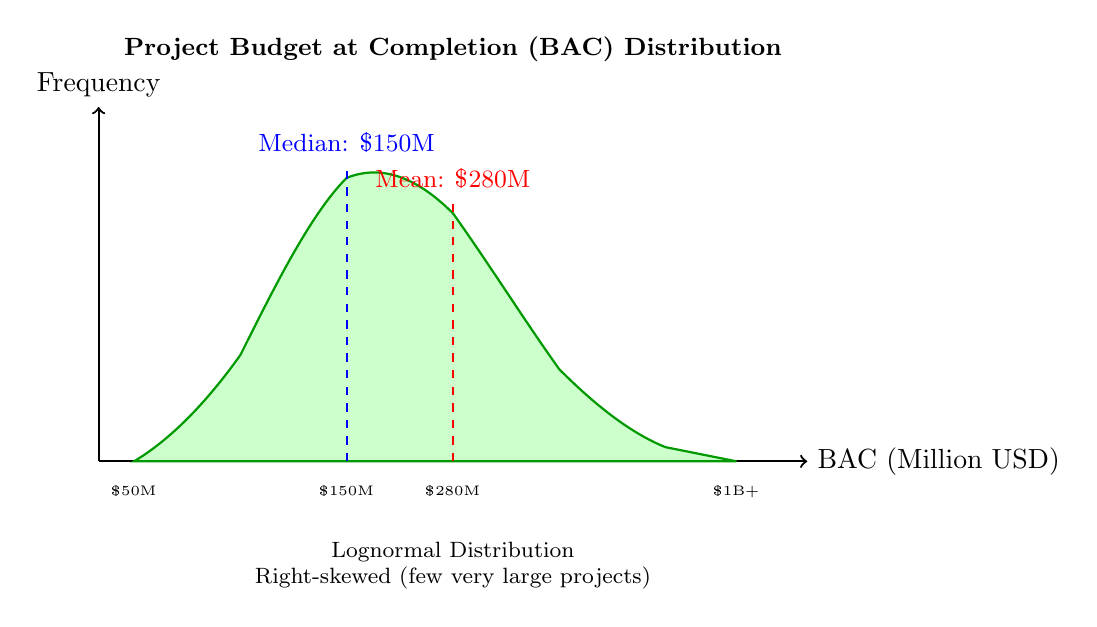
\begin{tikzpicture}[scale=0.9]
    % Axes
    \draw[thick, ->] (0,0) -- (10,0) node[right] {BAC (Million USD)};
    \draw[thick, ->] (0,0) -- (0,5) node[above] {Frequency};
    
    % Lognormal distribution (approximated)
    \draw[thick, green!60!black, fill=green!20] 
        (0.5,0) .. controls (1,0.3) and (1.5,0.8) .. (2,1.5)
        .. controls (2.5,2.5) and (3,3.5) .. (3.5,4.0)
        .. controls (4,4.2) and (4.5,4.0) .. (5,3.5)
        .. controls (5.5,2.8) and (6,2.0) .. (6.5,1.3)
        .. controls (7,0.8) and (7.5,0.4) .. (8,0.2)
        .. controls (8.5,0.1) .. (9,0) -- cycle;
    
    % Median line
    \draw[thick, blue, dashed] (3.5,0) -- (3.5,4.2) node[above] {\small Median: \$150M};
    
    % Mean line
    \draw[thick, red, dashed] (5,0) -- (5,3.7) node[above] {\small Mean: \$280M};
    
    % X-axis labels
    \node[below] at (0.5,-0.2) {\tiny \$50M};
    \node[below] at (3.5,-0.2) {\tiny \$150M};
    \node[below] at (5,-0.2) {\tiny \$280M};
    \node[below] at (9,-0.2) {\tiny \$1B+};
    
    % Annotations
    \node[below, font=\footnotesize, align=center] at (5,-1) {
        Lognormal Distribution\\
        Right-skewed (few very large projects)
    };
    
    % Title
    \node[above, font=\small\bfseries] at (5,5.5) {Project Budget at Completion (BAC) Distribution};
\end{tikzpicture}
